\subsection{$70\degree$ Turn}

\subsubsection{Curved $70\degree$ Turn}

The optimized path of a $70\degree$ turn with a radius of $150$m is shown in Figure \ref{fig:turns_cur_70deg_pos}. Even though the camera centre points deviates more from the desired path than during the $45\degree$ turn, the result is still a smooth path with no big unwanted motions.

\begin{figure}
	\makebox[\textwidth][c]{
	\subfloat[UAV position][UAV position.]{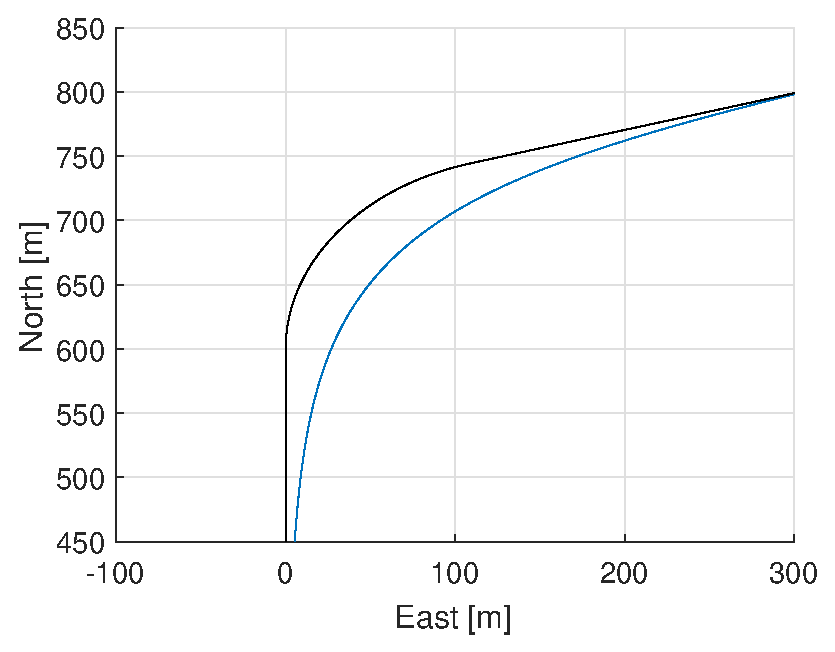
\includegraphics[width=0.5\textwidth, keepaspectratio=true]{../../results/opt/turns/curved/fig_70deg/uav_position.eps}}
	\qquad
	\subfloat[Camera position][Camera poistion.]{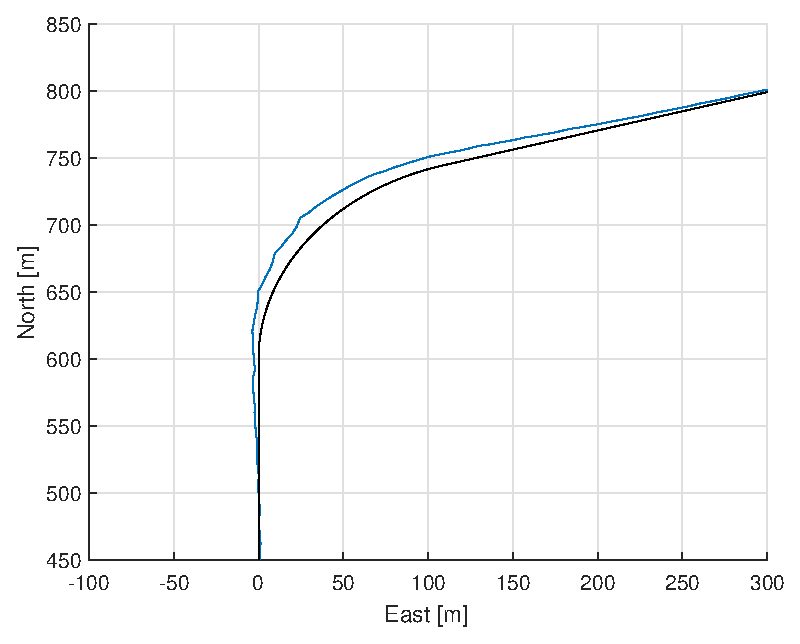
\includegraphics[width=0.5\textwidth, keepaspectratio=true]{../../results/opt/turns/curved/fig_70deg/camera_position.eps}}}
	\caption{Results of optimizing a curved $70\degree$ turn.}
	\label{fig:turns_cur_70deg_pos}
\end{figure}


\subsubsection{Linear $70\degree$ Turn}

Optimizing a path containing a $70\degree$ linear turn returns a very different result than for the curved turn. As can be seen in Figure \ref{fig:turns_lin_70deg_pos1}, the MPC is not able to achieve stable flight throughout the turn. The reason for this is similar to the reason why optimization with a short horizon length fails: the optimization tries banking the aircraft left to track the path, instead of cutting the corner. In this case the banking happens before the UAV have reached the corner as a result of the optimization "foreseeing" that it cannot keep tracking the path.

\begin{figure}
	\makebox[\textwidth][c]{
	\subfloat[UAV position][UAV position.]{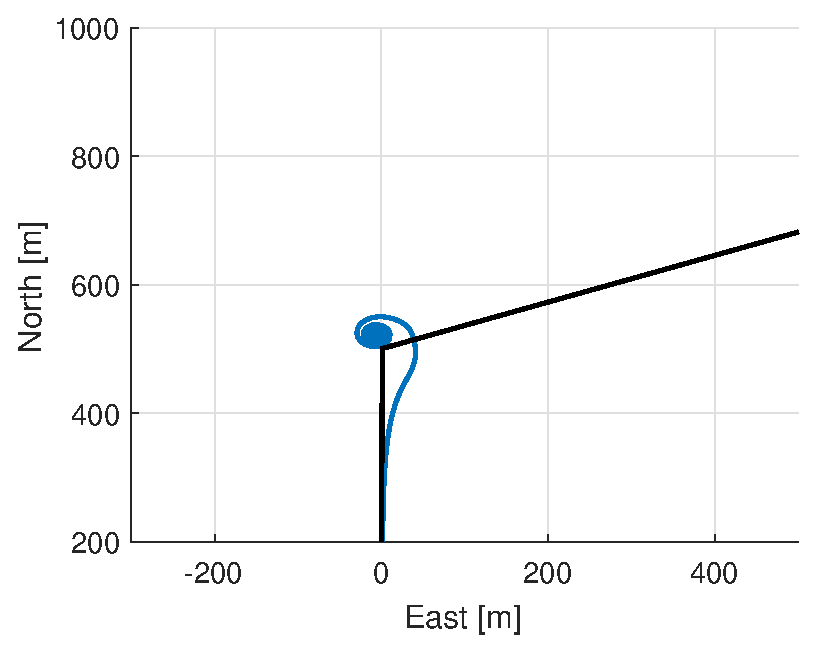
\includegraphics[width=0.5\textwidth, keepaspectratio=true]{../../results/opt/turns/linear/fig_70deg/uav_position_1.eps}}
	\qquad
	\subfloat[Camera position][Camera poistion.]{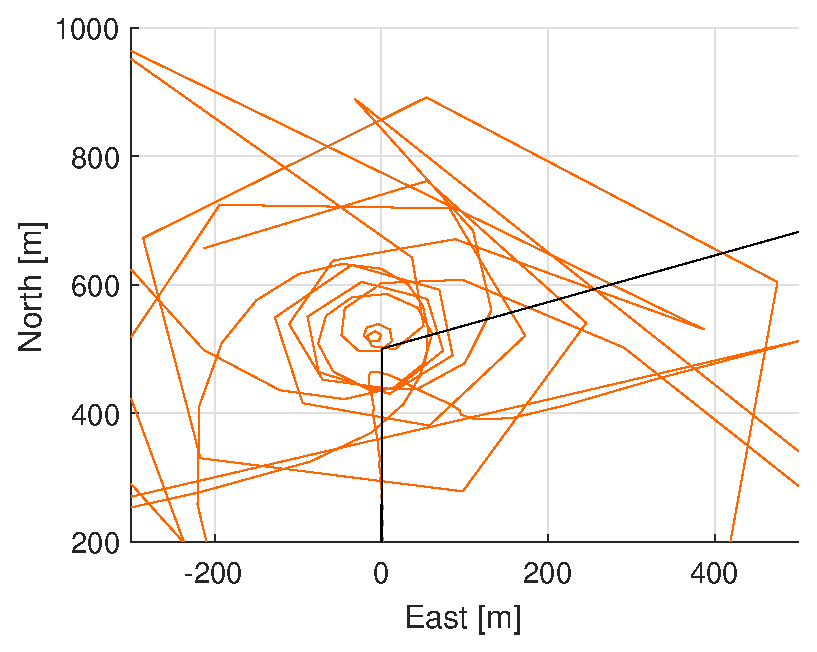
\includegraphics[width=0.5\textwidth, keepaspectratio=true]{../../results/opt/turns/linear/fig_70deg/camera_position_1.eps}}}
	\caption{Results of optimizing a linear $70\degree$ turn with $10^{-1}$ weight on camera position.}
	\label{fig:turns_lin_70deg_pos1}
\end{figure}

In an attempt to achieve stable flight throughout the turn, the weighting on camera position in the objective function was reduced. The result of changing the weighting from $10^{-1}$ to $10^{-3}$ can be seen in Figure \ref{fig:turns_lin_70deg_pos3}. This tuning results in a stable flight, but the path tracking is not as precise and smooth as for the $45\degree$ turn. In addition the resulting camera path consists of several loops. This occurs as a combination of both the roll angle and pitch angle changes at the same time.

\begin{figure}
	\makebox[\textwidth][c]{
	\subfloat[UAV position][UAV position.]{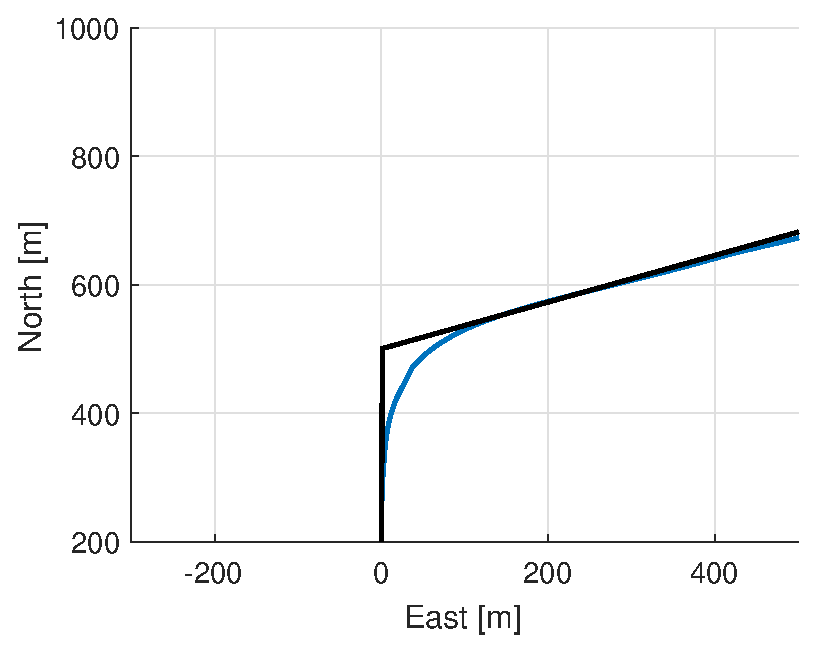
\includegraphics[width=0.5\textwidth, keepaspectratio=true]{../../results/opt/turns/linear/fig_70deg/uav_position_3.eps}}
	\qquad
	\subfloat[Camera position][Camera poistion.]{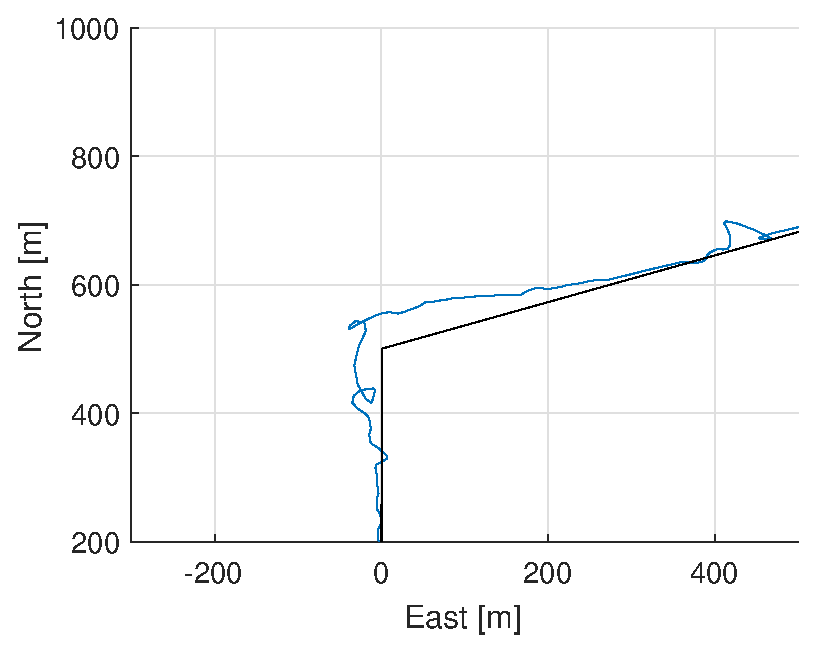
\includegraphics[width=0.5\textwidth, keepaspectratio=true]{../../results/opt/turns/linear/fig_70deg/camera_position_3.eps}}}
	\caption{Results of optimizing a linear $70\degree$ turn with $10^{-3}$ weight on camera position.}
	\label{fig:turns_lin_70deg_pos3}
\end{figure}

A third attempt on a linear $70\degree$ turn was made, this time with a weighting on the camera position of $10^{-5}$. As can be seen in Figure \ref{fig:turns_lin_70deg_pos5}, this results in a stable flight. The path tracking on the other hand is poor. With this tuning, the weight on the camera position is so much lower than on the other states included in the objective function so that the MPC finds a path that do not track the path returns the lowest cost. The optimization still makes some attempts to track the path, but ends up "swinging" the camera quickly past the path.

\begin{figure}
	\makebox[\textwidth][c]{
	\subfloat[UAV position][UAV position.]{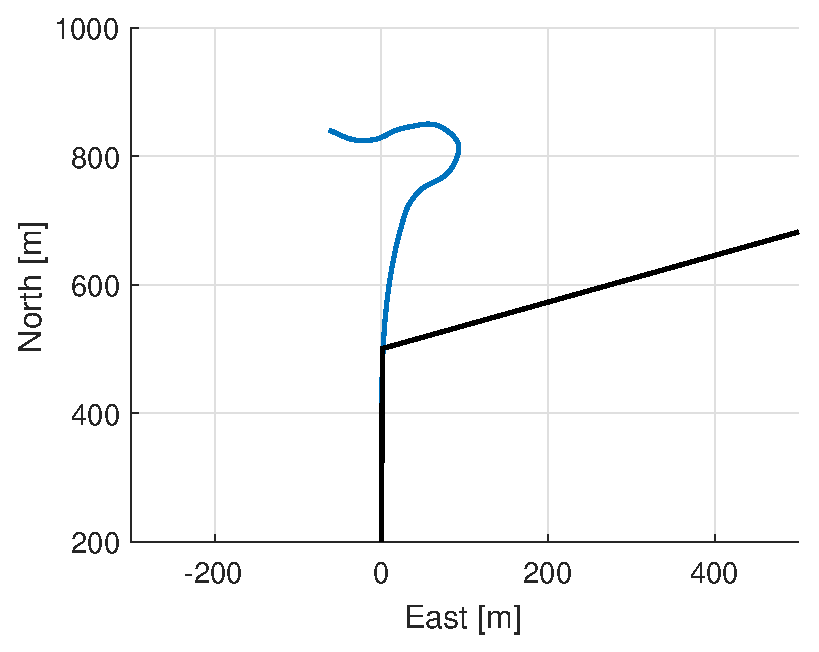
\includegraphics[width=0.5\textwidth, keepaspectratio=true]{../../results/opt/turns/linear/fig_70deg/uav_position_5.eps}}
	\qquad
	\subfloat[Camera position][Camera poistion.]{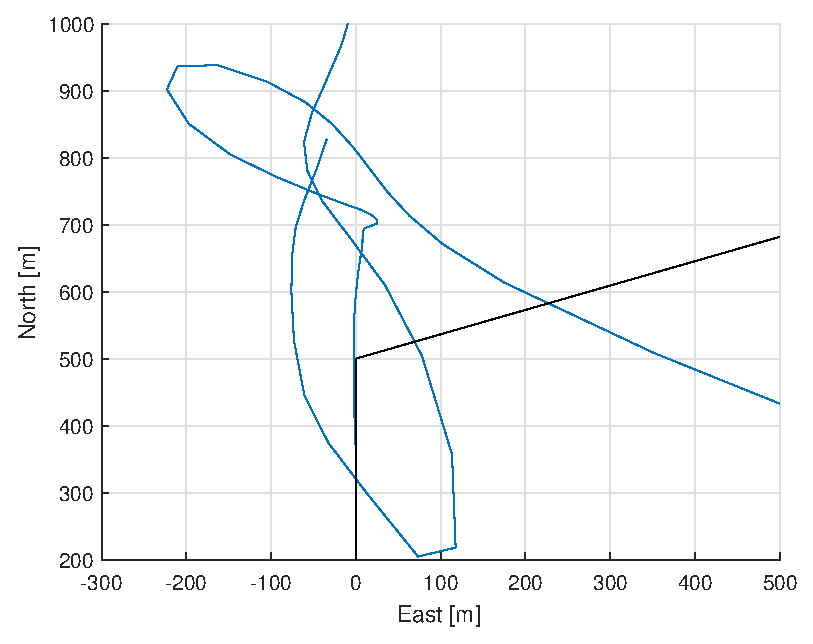
\includegraphics[width=0.5\textwidth, keepaspectratio=true]{../../results/opt/turns/linear/fig_70deg/camera_position_5.eps}}}
	\caption{Results of optimizing a linear $70\degree$ turn with $10^{-5}$ weight on camera position.}
	\label{fig:turns_lin_70deg_pos5}
\end{figure}